
\subsection{Implicit Method}
\begin{frame}{Implicit Method}

\begin{block}{}
   $$ \begin{array}{l}
   \text{Dla } t = 100, h = \frac{1}{100} \\
   \end{array}$$
 \end{block}
 
z $\lambda \leq \frac{1}{2} \Rightarrow \Delta t = k \leq \frac{1}{2}(\frac{1}{100})^2 = 5 \cdot 10^{-5}$  \\
  \begin{alertblock}{Problem}
    Dla znalezienia rozwiązania dla $t = 100$ potrzeba $2 \cdot 10^6$ wierszy!
  \end{alertblock}
Rozwiązaniem jest zmiania podstawowego równania: 
       \centerline{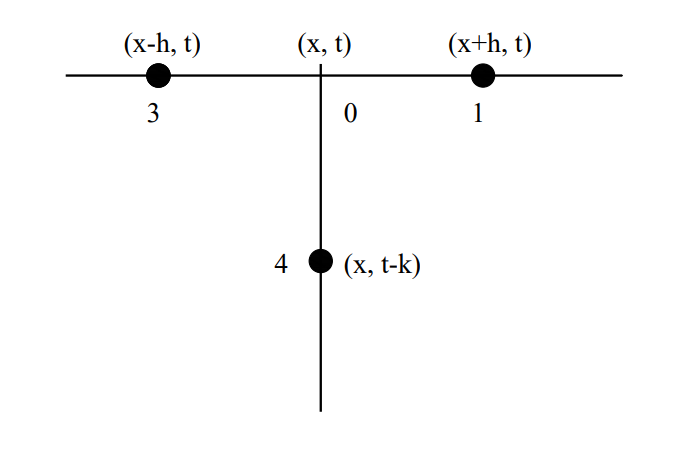
\includegraphics[width = 0.5 \linewidth]{img/23/implicit}}
\end{frame}

\begin{frame}
\begin{equation}\frac{u(x-h,t) - 2 \cdot u(x,t) + u(x+h, t)}{h^2} = \frac{u(x,t) - u(x,t - k)}{k}\end{equation}
co możemy zapisać: \begin{equation}\lambda \cdot u(x-h,t) - (1+2 \cdot \lambda)u(x,t) + \lambda \cdot u(x+h,t) = -u(x,t-k)\end{equation} 
albo:\begin{equation}\lambda \cdot u_3 - (1+2\cdot \lambda) \cdot u_0 + \lambda \cdot u_1 = - u_4 \rightarrow \text{stabilny dla wszystkich } \lambda\end{equation}

\begin{block}{}
Tym razem do wyznaczenia rozwiązań dla każdego wiersza trzeba
rozwiązać układ równań liniowych z macierzą trójdiagonalną, diagonalnie dominującą.
\end{block}

\end{frame}